\documentclass{article}
\usepackage[utf8]{inputenc}
\usepackage[T1]{fontenc}
\usepackage[french]{babel}
\usepackage{graphicx}

\title{Lancer de rayon - Première partie}
\author{Simon CHOPIN \and Marie-Morgane PAUMARD}
\date{\today}

\begin{document}

\maketitle
\tableofcontents
\begin{abstract}
><
\end{abstract}

\paragraph{Mots-clef}
lancer de rayon ; raytracing ; raycasting ; C++ ; réflexion ; réfraction ; backend camera.

\section{Introduction}
\subsection{Présentation}
Le lancer de rayon est une technique de synthèse d’image. Il s’agit de calculer
les trajectoires des rayons lumineux depuis la caméra jusqu’à l’objet, puis de
l’objet jusqu’à la source.
Nous avons traité ce projet selon l'approche de Arthur \textsc{Appel} (1968) :
il n'y a ni réflexion ni réfraction, qui seront ajoutées en seconde partie du
projet.

\subsection{Objectifs}
Ce troisième projet de programmation nous a permis de mettre en pratique nos
acquis en C++.

\subsection{Modèle physique}
On se place dans le cadre de l'optique géométrique : il n'y a pas
d'interférences ou de diffraction. Les sphères sont placées dans le vide : il
n'y a donc pas de diffusion, les ombres seront tranchées. Chaque source est
ponctuelle et monochromatique : la lumière blanche est modélisée par la somme
de sources monochromatiques.

\section{Implémentation de base}


\section{Améliorations}
\subsection{Améliorations réalisées}
\subsubsection{Objets non sphériques}
Pour pouvoir observer les ombres portées, nous avons insérés des plans dans
notre rendu. Il s'agit d'une classe similaire à la classe sphère : elle hérite
également de la classe objet.

Sur la figure ci-dessous, on voit deux plans (l'un jaune, l'autre violet) et
trois sphères. Il y a trois sources monochromatiques.

\begin{center}
  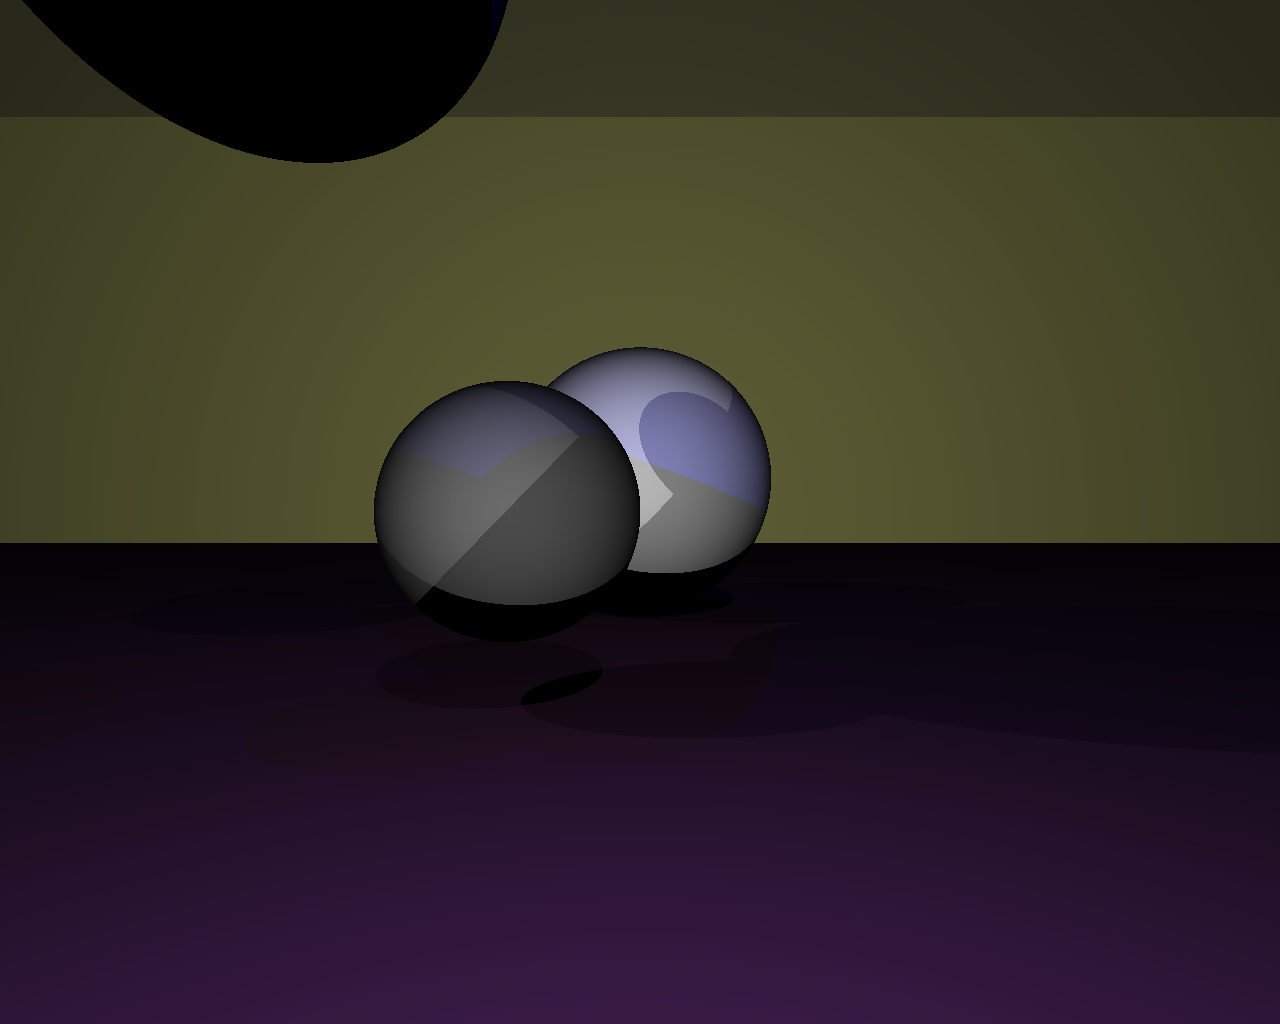
\includegraphics[scale=0.2]{img/screenshot.png}
\end{center}


\subsubsection{Backend camera}

\subsection{Exemples d'améliorations aisément implémentables}
\subsubsection{Gestion des matériaux : la réfraction}
La réfraction est le phénomène de déviation du rayon lumineux qui se produit
lors d’un changement de milieux transparents d’indices différents : sa
trajectoire est modifiée selon sa longueur d'onde.

\begin{center}
  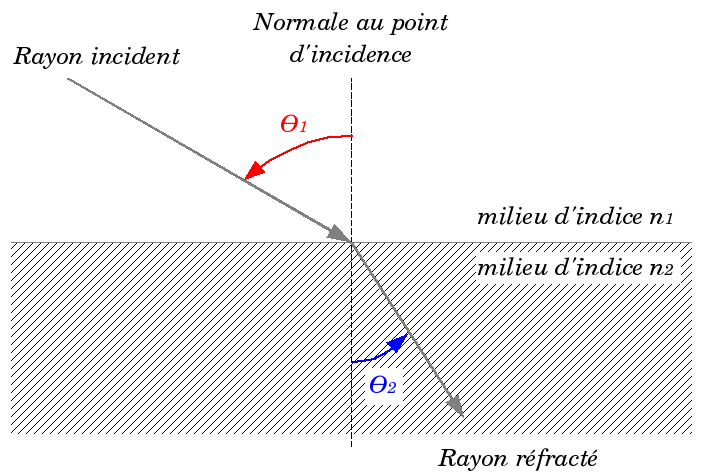
\includegraphics[scale=0.5]{img/refraction.png}
\end{center}

\paragraph{Implémentation}
Dans notre programme, il est aisé de mettre en œubre la réflexion. Pour ce faire
, il suffit de munir la classe objet de l'indice du milieu et d'un coefficient
de transmission.

L'indice du milieu $n$ permet de calculer la déviation du rayon, selon la loi de
\textsc{Snell-Descartes} : $n_i \sin i = n_r \sin r$, où $i$ (respectivement $r$)
est l'angle entre la normale et le rayon incident (respectivement réfléchi). $n$
vaut 1 dans le vide et représente la vitesse du rayon dans le milieu divisée par
la célérité de la lumière.

Le coefficient de transmission $t$ nous permet de calculer l'intensitée lumineuse
transmise par le milieu. Si $t=1$, le milieu se comporte comme le vide ; si $t=0$,
il réagit comme un milieu opaque, ce qui correspond au cas étudié dans cette
première partie du projet. On a : $t=\frac{2n_i}{n_i + n_r}$.

\paragraph{Milieux}
Cette extension permet de se placer dans un milieu autre que le vide. On peut
ainsi imaginer vouloir traiter le milieu comme un objet : il disposerait d'une
couleur et de coefficients de transmission et réflexion. On peut par exemple se
placer dans un gaz très dense, dans lequel les objets lointains ne sont plus que
de vagues formes désaturées.

\subsubsection{Gestion des matériaux : la réflexion}
La réflexion est un phénomène de déviation du rayon lumineux : en arrivant
sur une surface, une partie du rayon est renvoyé.

\begin{center}
  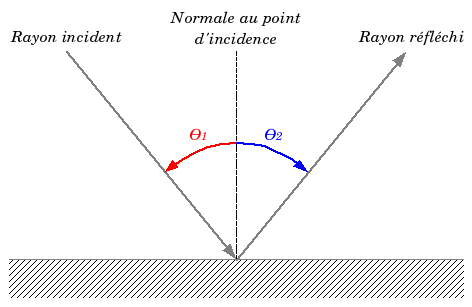
\includegraphics[scale=0.5]{img/reflexion.png}
\end{center}

\paragraph{Implémentation}
Pour implémenter la réflexion, on muni la classe objet de l'indice du milieu et
d'un coefficient de réflexion $r$.

Ce coefficient est obtenu par la loi : $r= \frac{n_i - n_r}{n_i + n_r}$. On a
donc $1+r=t$.

\section{Conclusion}

\appendix
\section{Bibliographie}

\end{document}
